\newpage
\section{236. 二叉树的最近公共祖先}
\label{leetcode:236}

\subsection{题目}

给定一个二叉树, 找到该树中两个指定节点的最近公共祖先。

百度百科中最近公共祖先的定义为:``对于有根树 T 的两个结点 p、q,
最近公共祖先表示为一个结点 x,满足 x 是 p、q 的祖先且 x 的深度尽可能大
(一个节点也可以是它自己的祖先)。''

例如,给定如下二叉树:  root = [3,5,1,6,2,0,8,null,null,7,4]

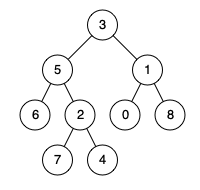
\includegraphics[width=60mm,height=60mm]{images/leetcode/leetcode_236_binarytree.png}

\textbf{示例 1}:

\begin{verbatim}
  输入: root = [3,5,1,6,2,0,8,null,null,7,4], p = 5, q = 1
  输出: 3
  解释: 节点 5 和节点 1 的最近公共祖先是节点 3。
\end{verbatim}

\textbf{示例 2}:

\begin{verbatim}
  输入: root = [3,5,1,6,2,0,8,null,null,7,4], p = 5, q = 4
  输出: 5
  解释: 节点 5 和节点 4 的最近公共祖先是节点 5。
  因为根据定义最近公共祖先节点可以为节点本身。
\end{verbatim}

\textbf{说明}:

\begin{enumerate}
  \item 所有节点的值都是唯一的。
  \item p、q 为不同节点且均存在于给定的二叉树中。
\end{enumerate}

\subsection{参考题解}

\subsubsection{JavaScript}

\begin{verbatim}
/**
 * Definition for a binary tree node.
 * function TreeNode(val) {
 *     this.val = val;
 *     this.left = this.right = null;
 * }
 */
/**
 * @param {TreeNode} root
 * @param {TreeNode} p
 * @param {TreeNode} q
 * @return {TreeNode}
 */
var lowestCommonAncestor = function(root, p, q) {
  if (root === null || root === p || root === q) {
    return root;
  }
  let left = lowestCommonAncestor(root.left, p, q);
  let right = lowestCommonAncestor(root.right, p, q);
  if (left === null) { return right; }
  if (right === null) { return left; }
  return root;
};
\end{verbatim}

\subsubsection{Golang}

\begin{verbatim}
/**
* Definition for TreeNode.
* type TreeNode struct {
*     Val int
*     Left *ListNode
*     Right *ListNode
* }
*/
func lowestCommonAncestor(root, p, q *TreeNode) *TreeNode {
  if root == nil || root == p || root == q {
    return root
  }
  left := lowestCommonAncestor(root.Left, p, q)
  right := lowestCommonAncestor(root.Right, p, q)
  if left == nil {
    return right
  }
  if right == nil {
    return left
  }
  return root
}
\end{verbatim}
